\documentclass[aspectratio=1610]{beamer}

% ---------- Tema estilo "sidebar" (Berkeley) en verde oscuro ----------
\usetheme{Berkeley}
\usecolortheme{default}

\usepackage[spanish]{babel}
\usepackage[utf8]{inputenc}
\usepackage[T1]{fontenc}
\usepackage{booktabs}
\usepackage{graphicx}
\usepackage{amsmath}

% Paquetes para la decoración gráfica, sombras y posición absoluta
\usepackage{tikz}
\usetikzlibrary{shadows.blur, arrows.meta}

\graphicspath{{../Figuras/}}

% Paleta verde oscuro
\definecolor{unc verde}{RGB}{27,58,48}
\definecolor{unc verdeclaro}{RGB}{60,110,90}

\setbeamercolor{palette primary}{bg=unc verde,fg=white}
\setbeamercolor{palette secondary}{bg=unc verde,fg=white}
\setbeamercolor{palette tertiary}{bg=unc verde,fg=white}
\setbeamercolor{palette quaternary}{bg=unc verde,fg=white}
\setbeamercolor{structure}{fg=unc verde}
\setbeamercolor{title}{bg=unc verde,fg=white}
\setbeamercolor{frametitle}{bg=unc verde,fg=white}
\setbeamercolor{sidebar}{bg=unc verde}
\setbeamercolor{section in sidebar}{fg=white}
\setbeamercolor{section in sidebar shaded}{fg=unc verdeclaro}
\setbeamercolor{subsection in sidebar}{fg=white}
\setbeamercolor{subsection in sidebar shaded}{fg=unc verdeclaro}
\setbeamercolor{title in sidebar}{fg=white}
\setbeamercolor{author in sidebar}{fg=white}
\setbeamerfont{section in sidebar}{series=\bfseries}

% Título y datos de la presentación
\title[Fibra Óptica]{Introducción a las comunicaciones con fibra óptica}
\subtitle{Sistemas de Radiocomunicación -- Actividad 3}
\author[Arteaga, Baccino, Mendes Rosa, Monja]{\texorpdfstring{Arteaga Barrera, Cristian Eduardo \\ Baccino, Luca \\ Mendes Rosa, Agustín \\ Monja, Ernesto Joaquín}{Arteaga Barrera, Cristian Eduardo; Baccino, Luca; Mendes Rosa, Agustín; Monja, Ernesto Joaquín}}
\institute[FCEFyN -- UNC]{Facultad de Ciencias Exactas, Físicas y Naturales \\ Universidad Nacional de Córdoba}
\date{Córdoba, 2026}

\setbeamertemplate{navigation symbols}{}
\setbeamertemplate{footline}[frame number]

\begin{document}

% =====================================================
% ---------- Portada ----------
% =====================================================
\begin{frame}[plain]
  \begin{tikzpicture}[remember picture, overlay]
    \node[anchor=east, xshift=1.2cm, yshift=-0.5cm, opacity=0.65] at (current page.east) {
      
\includegraphics[height=0.9\paperheight]{decoracion_a.png}
    };
    \fill[unc verde] (current page.north west) rectangle ([yshift=-1.6cm]current page.north east);
    \node[
      fill=unc verde,
      text=white,
      rounded corners=3pt,
      blur shadow={shadow blur steps=5, shadow xshift=0pt, shadow yshift=-3pt, shadow opacity=40},
      inner sep=12pt,
      minimum width=0.88\paperwidth,
      align=center,
      font=\Large\bfseries
    ] at ([yshift=-2.6cm]current page.north) {
      Sistemas de Radiocomunicación \\ Actividad 3: Fibra Óptica
    };
    \node[anchor=center, text width=0.85\paperwidth, align=center] at ([yshift=-1.4cm]current page.center) {
      {\large\bfseries Introducción a las comunicaciones con fibra óptica}\\[0.25cm]
      {\normalsize Arteaga Barrera, Cristian Eduardo\\Baccino, Luca\\ Mendes Rosa, Agustín\\ Monja, Ernesto Joaquín}\\[0.25cm]
      {\small Facultad de Ciencias Exactas, Físicas y Naturales}\\[0.08cm]
      {\small Universidad Nacional de Córdoba}\\[0.25cm]
      {\small Córdoba, 2026}
    };
    \node[anchor=south] at ([yshift=0.1cm]current page.south) {
      
\includegraphics[height=1.2cm]{unc_fcefyn_logo.png}
    };
  \end{tikzpicture}
\end{frame}

% =====================================================
\begin{frame}{Contenido}
  \tableofcontents
\end{frame}

% =====================================================
\section[Intro]{Introducción}
\begin{frame}{Objetivos de la actividad}
  \textbf{Objetivo:} comprobar empíricamente los principios físicos y electrónicos de los enlaces ópticos con el kit educativo \textbf{Feedback EFO1101}.

  \vspace{0.4cm}
  \begin{columns}[T]
    \begin{column}{0.5\textwidth}
      \textbf{Modo analógico}
      \begin{itemize}
        \item A.1: audio por espacio libre
        \item A.2: audio por fibra óptica
        \item Propagación no guiada vs.\ guiada
      \end{itemize}
    \end{column}
    \begin{column}{0.5\textwidth}
      \textbf{Modo digital}
      \begin{itemize}
        \item D.1: código Morse y generador de ondas
        \item D.2: mediciones con osciloscopio
        \item Umbral de decisión, atenuación y ancho de banda
      \end{itemize}
    \end{column}
  \end{columns}
\end{frame}

\begin{frame}{Sistema de comunicación óptico}
  \begin{center}
    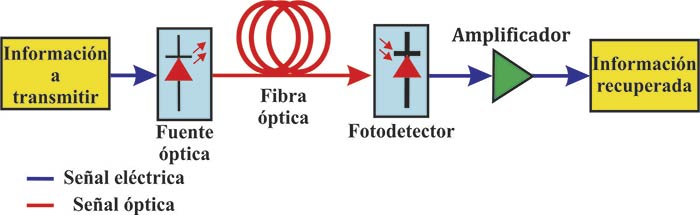
\includegraphics[width=0.85\textwidth]{diagrama1.png}
  \end{center}
  \begin{itemize}
    \item La fuente óptica convierte la señal eléctrica en luz.
    \item El canal puede ser el \textbf{espacio libre} (propagación no guiada) o la \textbf{fibra óptica} (propagación guiada).
    \item El fotodetector reconvierte la luz en una corriente eléctrica proporcional.
  \end{itemize}
\end{frame}

% =====================================================
\section[Teoría]{Marco teórico}
\begin{frame}{Reflexión total interna}
  \begin{columns}[T]
    \begin{column}{0.52\textwidth}
      \begin{itemize}
        \item Núcleo de $SiO_2$ con índice $n_1$, revestimiento con $n_2 < n_1$.
        \item Ley de Snell en la interfaz núcleo--revestimiento:
        \[ n_1 \sin\theta_i = n_2 \sin\theta_t \]
        \item Por encima del \textbf{ángulo crítico} no hay rayo refractado y toda la luz queda confinada:
        \[ \theta_c = \arcsin\left(\frac{n_2}{n_1}\right) \]
      \end{itemize}
    \end{column}
    \begin{column}{0.48\textwidth}
      \centering
      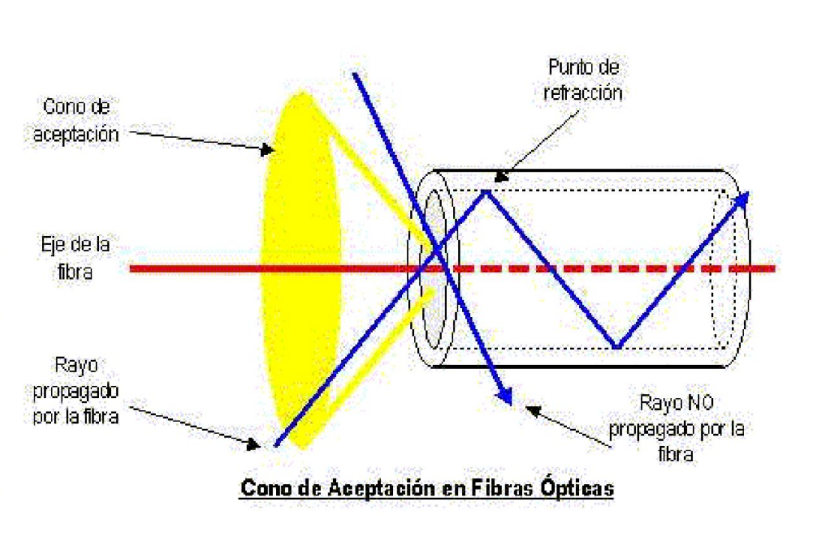
\includegraphics[width=\textwidth]{Cono.png}\\[0.1cm]
      \small Cono de aceptación
    \end{column}
  \end{columns}
  \vspace{0.2cm}
  \textbf{Apertura numérica:} capacidad de la fibra para captar la luz de la fuente
  \[ AN = \sin\alpha_{max} = n_1 \cos\theta_c = \sqrt{n_1^2 - n_2^2} \]
\end{frame}

\begin{frame}{Tipos de fibra y atenuación}
  \begin{columns}[T]
    \begin{column}{0.48\textwidth}
      \textbf{Según los modos de propagación}
      \begin{itemize}
        \item \textbf{Monomodo:} núcleo de 8 a 10\,$\mu$m, un solo modo.
        \item \textbf{Multimodo:} núcleo de 50\,$\mu$m o más; sufre \textbf{dispersión modal}, que limita distancia y velocidad.
      \end{itemize}
      \centering
      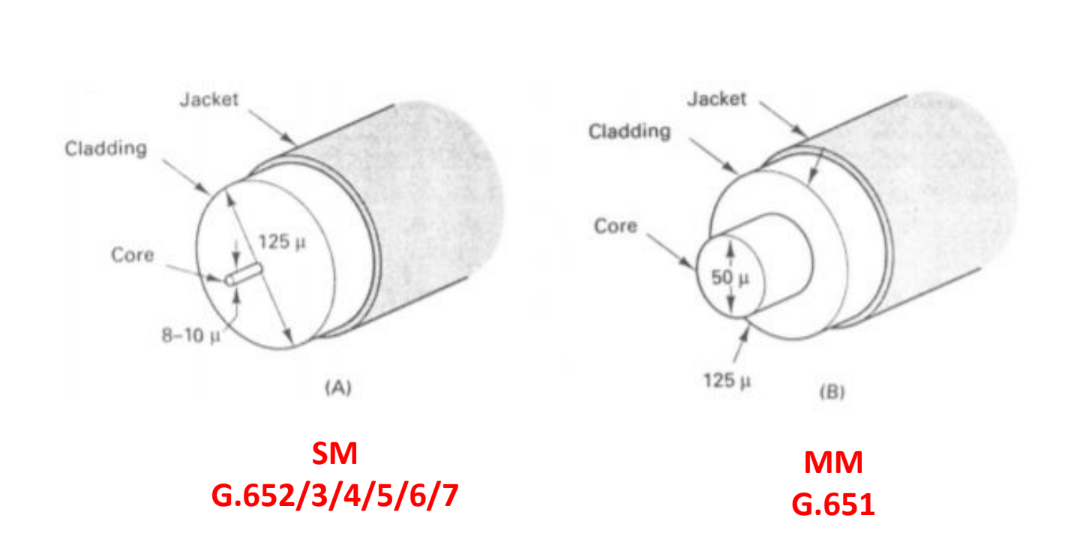
\includegraphics[width=0.9\textwidth]{Modos.png}
    \end{column}
    \begin{column}{0.52\textwidth}
      \textbf{Atenuación}
      \[ \alpha\,[dB] = 10 \log_{10}\left(\frac{P_{entrada}}{P_{salida}}\right) \]
      \centering
      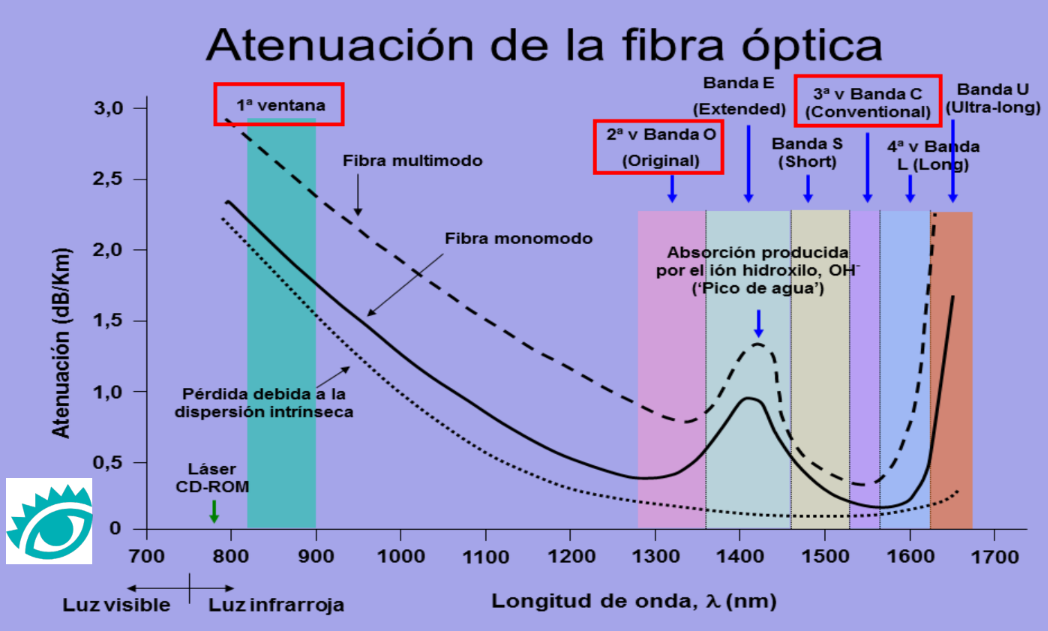
\includegraphics[width=0.9\textwidth]{Atenuacion.png}\\
      \raggedright
      \small El \textbf{pico de agua} (iones $OH^-$) se elimina en las fibras \emph{Low Water Peak}.
    \end{column}
  \end{columns}
\end{frame}

\begin{frame}{Modulación analógica y digital}
  \begin{columns}[T]
    \begin{column}{0.48\textwidth}
      \textbf{Analógica}
      \begin{itemize}
        \item La intensidad del LED es proporcional a la tensión de entrada.
        \item Se suma una continua (\emph{DC bias}) porque la luz no puede ser negativa.
      \end{itemize}
      \vspace{0.2cm}
      \textbf{Digital}
      \begin{itemize}
        \item El LED conmuta entre alta intensidad (``1'') y baja o nula (``0'').
        \item El receptor compara la señal con un \textbf{umbral de decisión}.
      \end{itemize}
    \end{column}
    \begin{column}{0.52\textwidth}
      \centering
      \begin{tikzpicture}[scale=0.85, font=\footnotesize]
        \draw[-{Stealth}] (0,0) -- (6.2,0) node[below left] {$t$};
        \draw[-{Stealth}] (0,0) -- (0,3.4) node[left] {$V_{RX}$};
        \draw[thick, unc verde] (0,0.3) -- (0.5,0.3) -- (0.5,2.6) -- (1.7,2.6) -- (1.7,0.3) -- (2.9,0.3) -- (2.9,2.6) -- (4.1,2.6) -- (4.1,0.3) -- (5.3,0.3) -- (5.3,2.6) -- (6,2.6);
        \draw[thick, red!70!black, dashed] (0,0.3) -- (0.5,0.3) -- (0.5,1.2) -- (1.7,1.2) -- (1.7,0.3) -- (2.9,0.3) -- (2.9,1.2) -- (4.1,1.2) -- (4.1,0.3) -- (5.3,0.3) -- (5.3,1.2) -- (6,1.2);
        \draw[thick, orange] (0,1.7) -- (6,1.7) node[right] {Umbral};
        \node[unc verde, anchor=west] at (0.1,3.1) {Fibra corta: supera el umbral};
        \node[red!70!black, anchor=west] at (0.1,-0.45) {Fibra larga: no lo supera};
      \end{tikzpicture}
    \end{column}
  \end{columns}
\end{frame}

% =====================================================
\section[Seguridad]{Seguridad}
\begin{frame}{Medidas de seguridad}
  \begin{columns}[T]
    \begin{column}{0.5\textwidth}
      \textbf{Riesgo óptico}
      \begin{itemize}
        \item Nunca mirar el extremo de una fibra o un emisor activo.
        \item No apuntar la fibra hacia la cara de otra persona.
        \item El infrarrojo no es visible: el ojo no activa el reflejo de parpadeo.
      \end{itemize}
    \end{column}
    \begin{column}{0.5\textwidth}
      \textbf{Riesgo mecánico y químico}
      \begin{itemize}
        \item Evitar curvaturas pronunciadas: la fibra puede astillarse.
        \item Las esquirlas de vidrio son casi invisibles: descartarlas en un recipiente adecuado.
        \item Alcohol isopropílico lejos de fuentes de calor.
      \end{itemize}
    \end{column}
  \end{columns}
\end{frame}

% =====================================================
\section[Kit]{Equipamiento}
\begin{frame}{Kit educativo Feedback EFO1101}
  \begin{columns}[T]
    \begin{column}{0.45\textwidth}
      \centering
      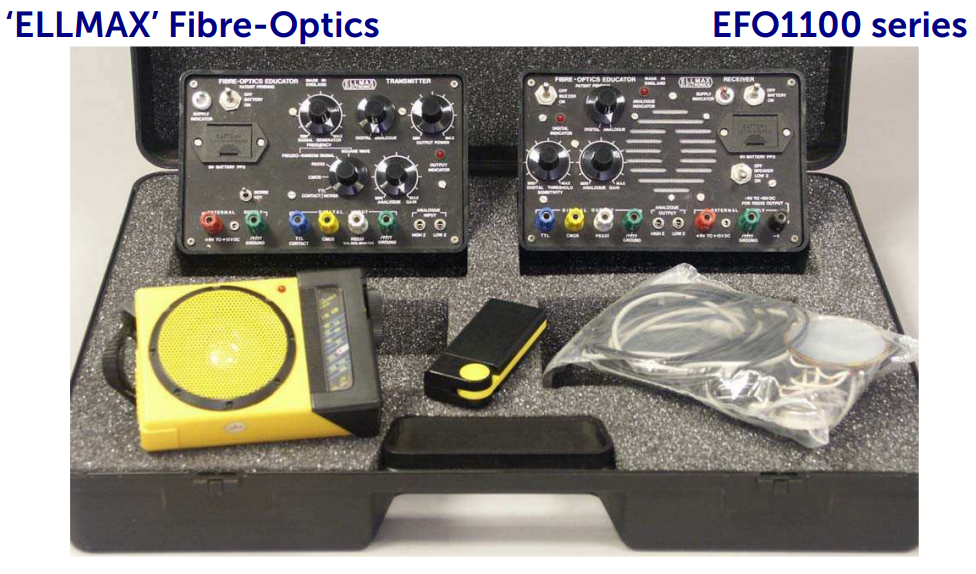
\includegraphics[width=\textwidth]{kit.png}\\[0.1cm]
      \small Transmisor, receptor, espejo y cables ópticos
    \end{column}
    \begin{column}{0.55\textwidth}
      \begin{itemize}
        \item \textbf{Transmisor:} LED de alta luminosidad (salida 10) y LED infrarrojo (salida 12).
        \item \textbf{Receptor:} fotodiodo, altavoz y buzzer.
        \item Modos analógico y digital seleccionables.
        \item Alimentación externa de 9 a 15\,V.
        \item Cables ópticos corto y largo.
        \item Osciloscopio Tektronix serie TDS.
      \end{itemize}
    \end{column}
  \end{columns}
\end{frame}

\begin{frame}{Elementos de control}
  \begin{columns}[c]
    \begin{column}{0.5\textwidth}
      \centering
      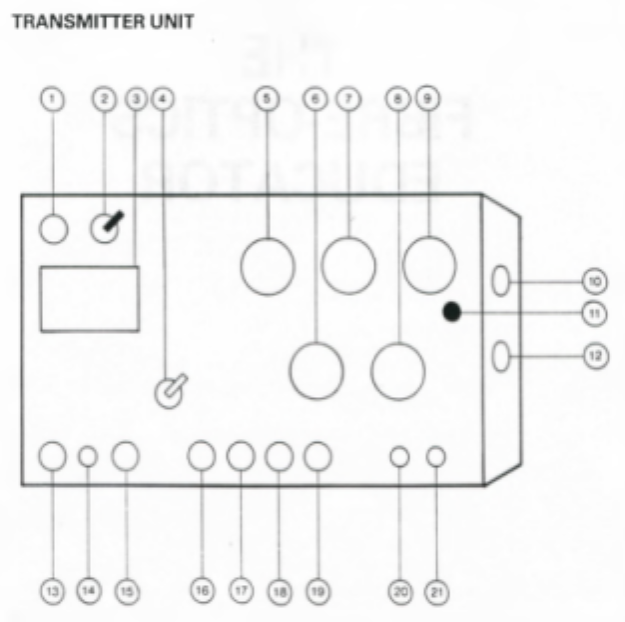
\includegraphics[width=0.85\textwidth]{Transmisor.png}\\[0.1cm]
      \small (a) Transmisor
    \end{column}
    \begin{column}{0.5\textwidth}
      \centering
      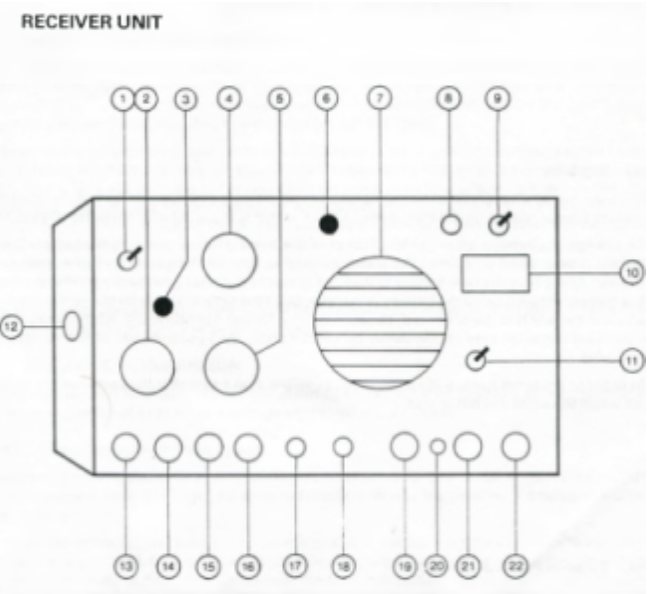
\includegraphics[width=0.9\textwidth]{Receptor.png}\\[0.1cm]
      \small (b) Receptor
    \end{column}
  \end{columns}
\end{frame}

% =====================================================
\section[Analógico]{Modo analógico}
\begin{frame}{A.1: Audio por espacio libre}
  \begin{columns}[T]
    \begin{column}{0.45\textwidth}
      \begin{itemize}
        \item Transmisor y receptor enfrentados a $\approx 50$\,cm.
        \item Audio a la entrada analógica (borne 21).
        \item Al tapar el LED visible el audio continúa: la información viaja por \textbf{infrarrojo}.
        \item Con el transmisor a $90^\circ$, el \textbf{espejo} redirige el haz y se recupera el audio.
      \end{itemize}
    \end{column}
    \begin{column}{0.55\textwidth}
      \centering
      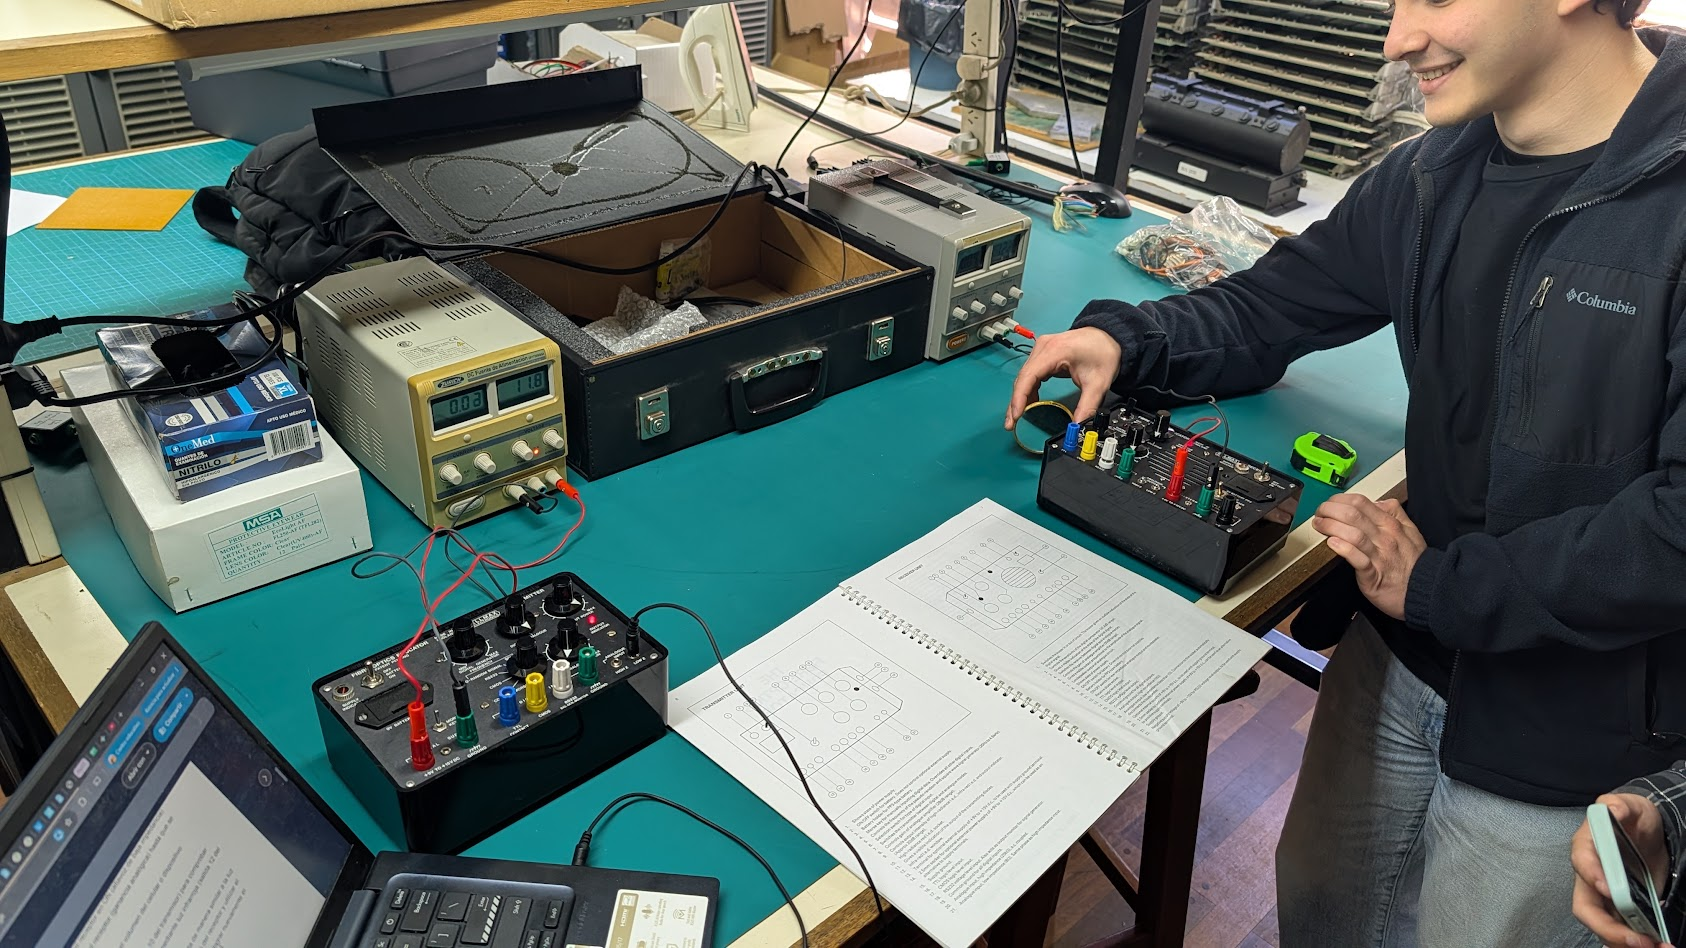
\includegraphics[width=\textwidth]{espejo.png}\\[0.1cm]
      \small Reflexión del haz infrarrojo con el espejo
    \end{column}
  \end{columns}
  \vspace{0.2cm}
  \centering
  \textbf{Resultado:} el infrarrojo obedece la ley de reflexión igual que la luz visible.
\end{frame}

\begin{frame}{A.2: Audio por fibra óptica}
  \begin{columns}[c]
    \begin{column}{0.5\textwidth}
      \centering
      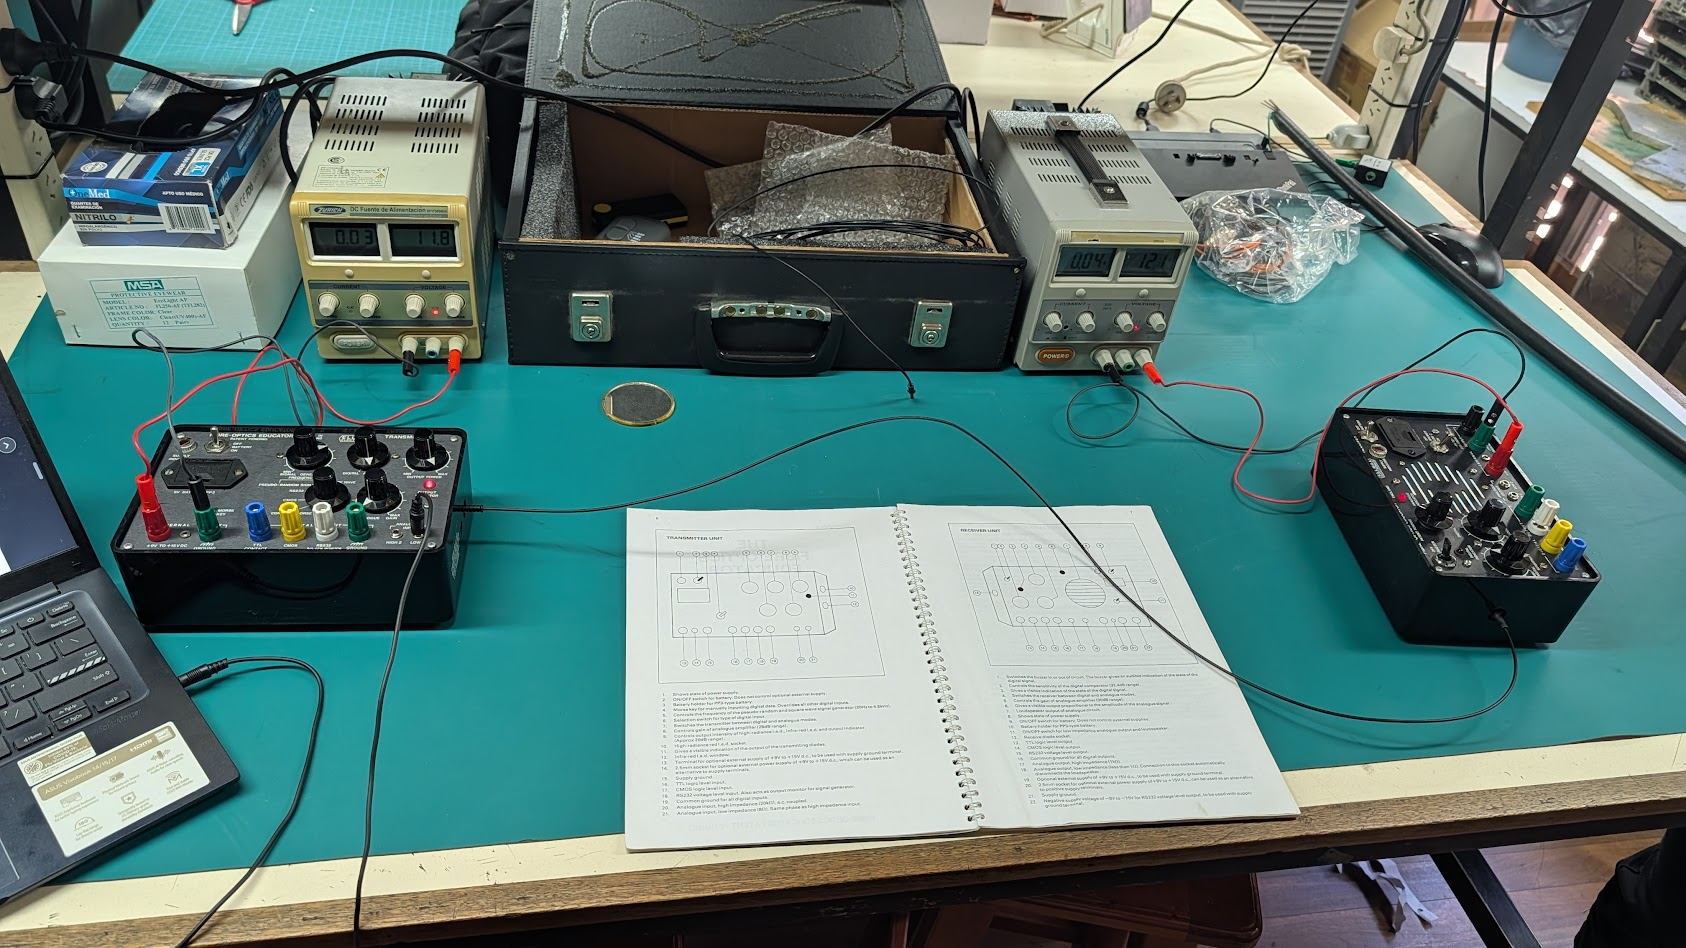
\includegraphics[height=0.33\textheight]{A2_corto.png}\\
      \small (a) Fibra corta\\[0.1cm]
      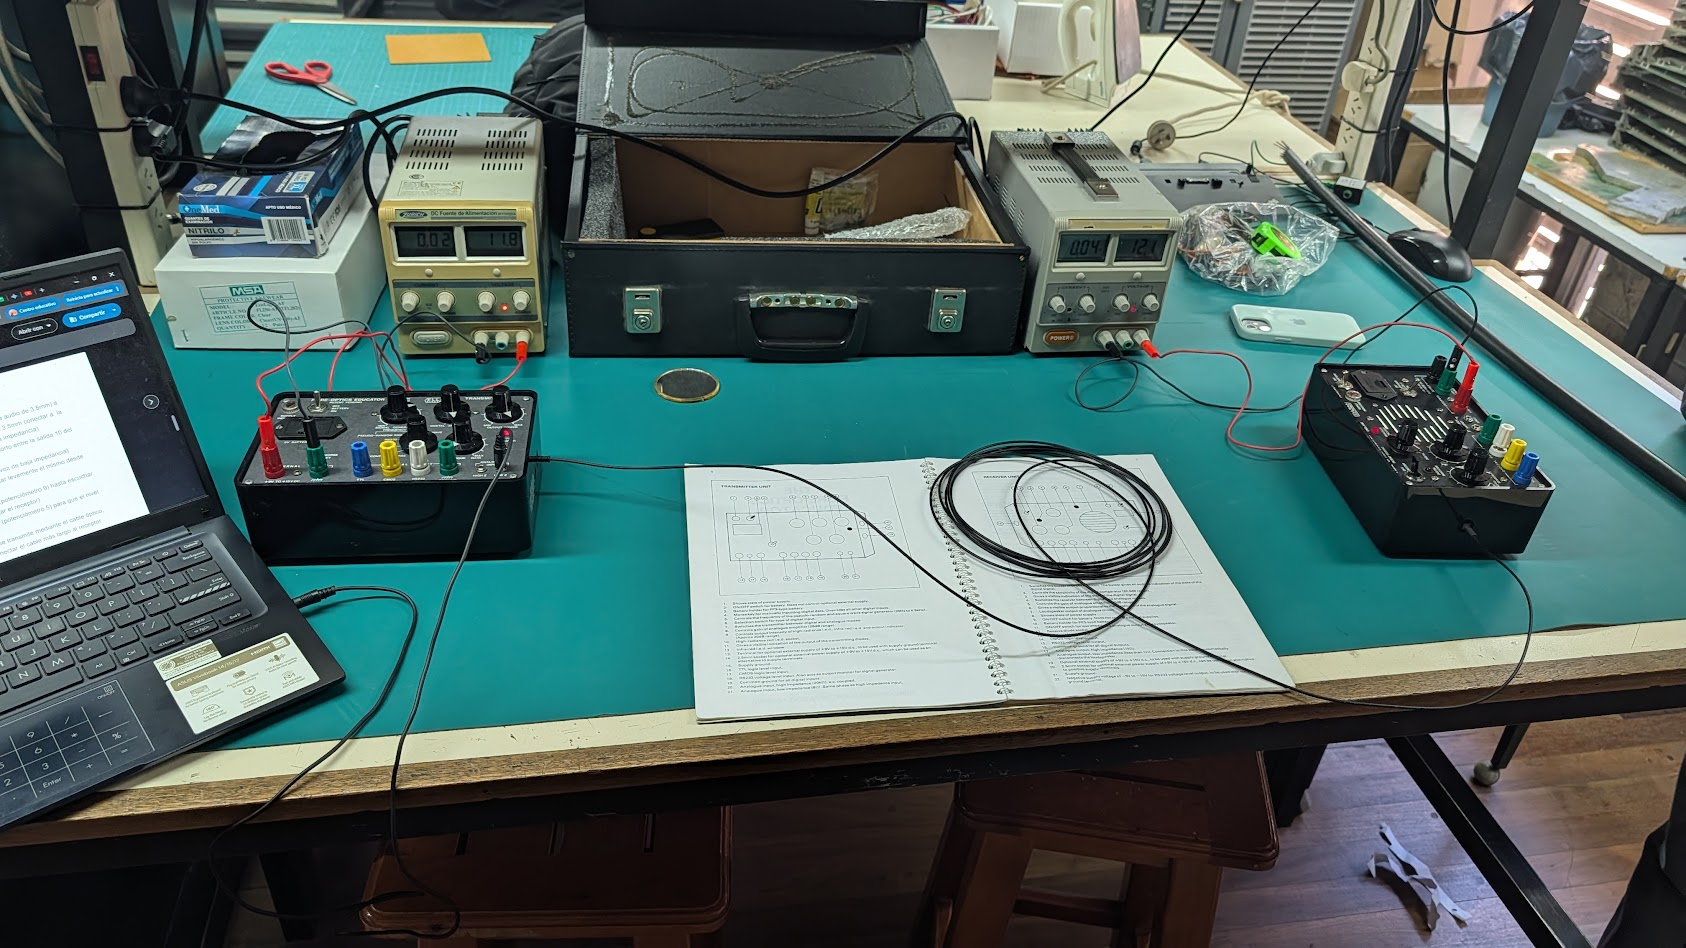
\includegraphics[height=0.33\textheight]{A2_largo.png}\\
      \small (b) Fibra larga
    \end{column}
    \begin{column}{0.5\textwidth}
      \centering
      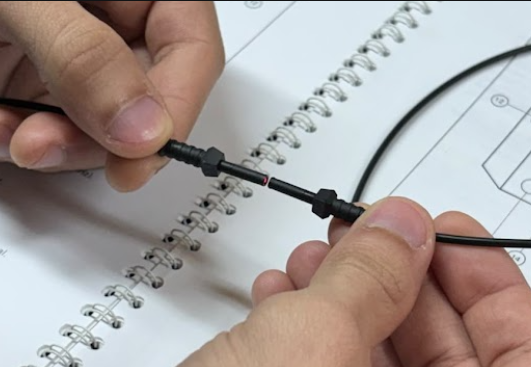
\includegraphics[height=0.33\textheight]{1.png}\\
      \small (c) Extremos de fibras enfrentados\\[0.1cm]
      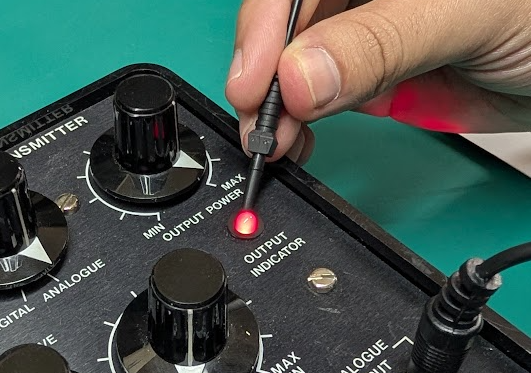
\includegraphics[height=0.33\textheight]{salida.png}\\
      \small (d) Indicador de salida (LED 11)
    \end{column}
  \end{columns}
\end{frame}

\begin{frame}{A.2: Observaciones}
  \begin{itemize}
    \item Con la misma configuración, el audio se escucha \textbf{mucho más fuerte} que por espacio libre.
    \item Fue necesario \textbf{reducir la potencia del transmisor} para no saturar el fotodetector.
    \item Al enfrentar manualmente dos fibras, la señal pasa, pero con menor nivel que con los conectores.
  \end{itemize}

  \vspace{0.3cm}
  \begin{block}{¿Por qué?}
    \begin{itemize}
      \item \textbf{Espacio libre:} el haz diverge y la potencia por unidad de área decae con la distancia.
      \item \textbf{Fibra óptica:} la reflexión total interna confina la luz y la guía hasta el área activa del fotodetector.
      \item \textbf{Acople manual:} desalineación y separación entre núcleos agregan pérdidas.
    \end{itemize}
  \end{block}
\end{frame}

% =====================================================
\section[Digital]{Modo digital}
\begin{frame}{D.1: Morse y generador de ondas}
  \begin{itemize}
    \item Con el pulsador \textbf{Morse} se verificó la transmisión digital por la fibra corta.
    \item Sin fibra, ajustando el \textbf{umbral} se logró detectar la \textbf{luz ambiente} como señal: el receptor sólo decide si la luz supera el umbral.
    \item Con las señales \textbf{pseudoaleatoria} y \textbf{cuadrada}, el buzzer reproduce el tono de la señal recibida.
    \item Al aumentar la frecuencia:
    \begin{itemize}
      \item el tono del buzzer se vuelve más agudo;
      \item el parpadeo del LED indicador deja de percibirse y se ve una luz continua (persistencia de la visión).
    \end{itemize}
  \end{itemize}
\end{frame}

\begin{frame}{D.2: Mediciones con osciloscopio}
  \begin{columns}[T]
    \begin{column}{0.4\textwidth}
      \begin{itemize}
        \item CH1: señal del transmisor.
        \item CH2: salida del receptor.
        \item Ambas señales \textbf{en fase}, sin inversión.
        \item La salida del receptor es una señal \textbf{regenerada}: el comparador la lleva a niveles cercanos a la alimentación.
      \end{itemize}
    \end{column}
    \begin{column}{0.6\textwidth}
      \centering
      \begin{tabular}{lcc}
        \toprule
        & \textbf{20,6 Hz} & \textbf{4,75 kHz} \\
        \midrule
        CH1 (TX) $V_{pp}$ & 316 mV & 372 mV \\
        CH2 (RX) $V_{pp}$ & 14,7 V & 10,5 V \\
        \bottomrule
      \end{tabular}\\[0.3cm]
      \small Rango de frecuencias del generador:\\ de 20,6 Hz a 4,75 kHz
    \end{column}
  \end{columns}
\end{frame}

\begin{frame}{D.2: Respuesta en los extremos de frecuencia}
  \begin{columns}[T]
    \begin{column}{0.5\textwidth}
      \centering
      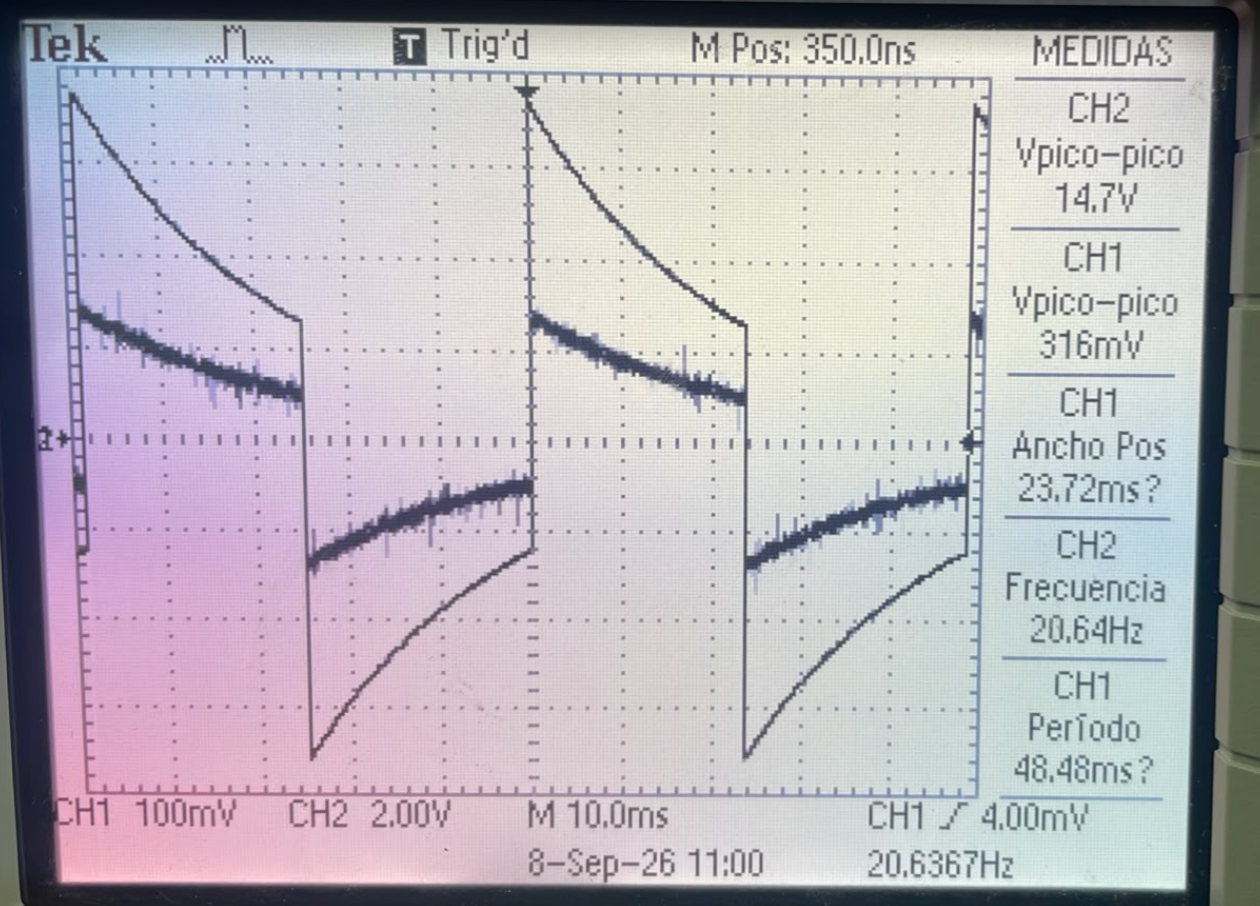
\includegraphics[width=0.95\textwidth]{20hz.png}\\
      \small (a) 20,6 Hz: caída del nivel en cada semiciclo
    \end{column}
    \begin{column}{0.5\textwidth}
      \centering
      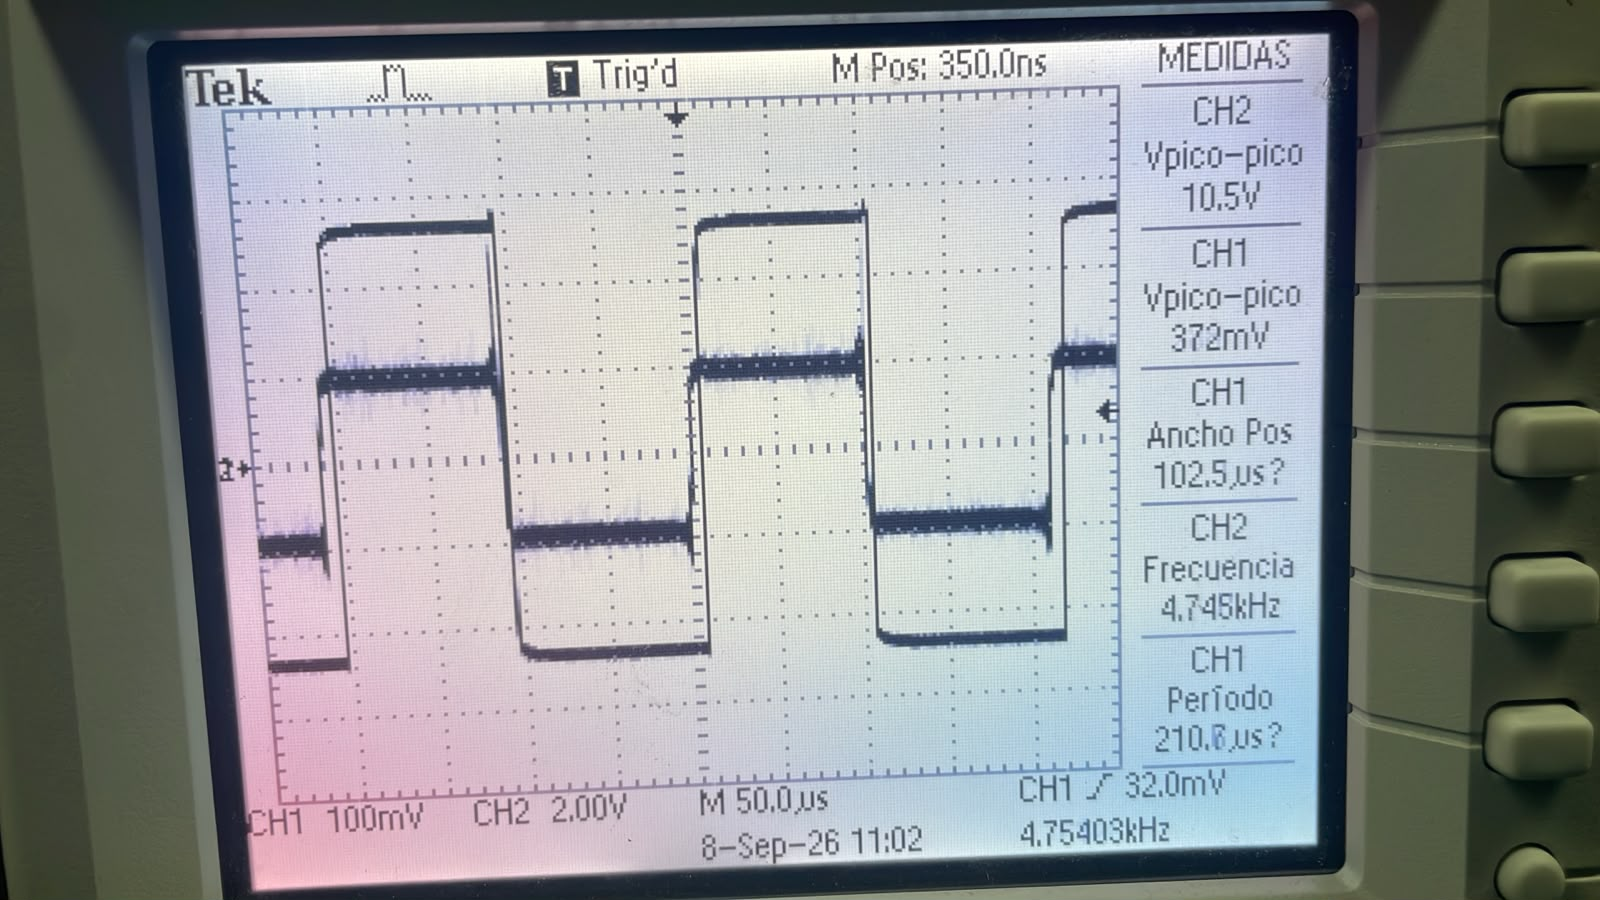
\includegraphics[width=\textwidth]{4khz.png}\\
      \small (b) 4,75 kHz: flancos redondeados
    \end{column}
  \end{columns}
  \vspace{0.2cm}
  \begin{itemize}
    \item \textbf{Baja frecuencia:} comportamiento pasa-altos por el acoplamiento en alterna (capacitores que bloquean la continua).
    \item \textbf{Alta frecuencia:} comportamiento pasa-bajos por la capacitancia del circuito y del fotodiodo, que limita los tiempos de conmutación.
  \end{itemize}
\end{frame}

\begin{frame}{D.2: Umbral de decisión y atenuación}
  \begin{columns}[T]
    \begin{column}{0.45\textwidth}
      \begin{enumerate}
        \item Con la fibra corta, se ajustó el umbral (potenciómetro 2) al límite de recepción.
        \item Se reemplazó por la fibra larga, sin tocar el umbral.
        \item La mayor atenuación hace que la señal no supere el umbral: \textbf{la salida del receptor desaparece}.
      \end{enumerate}
      \vspace{0.2cm}
      \small Demuestra que la fibra larga atenúa más que la corta.
    \end{column}
    \begin{column}{0.55\textwidth}
      \centering
      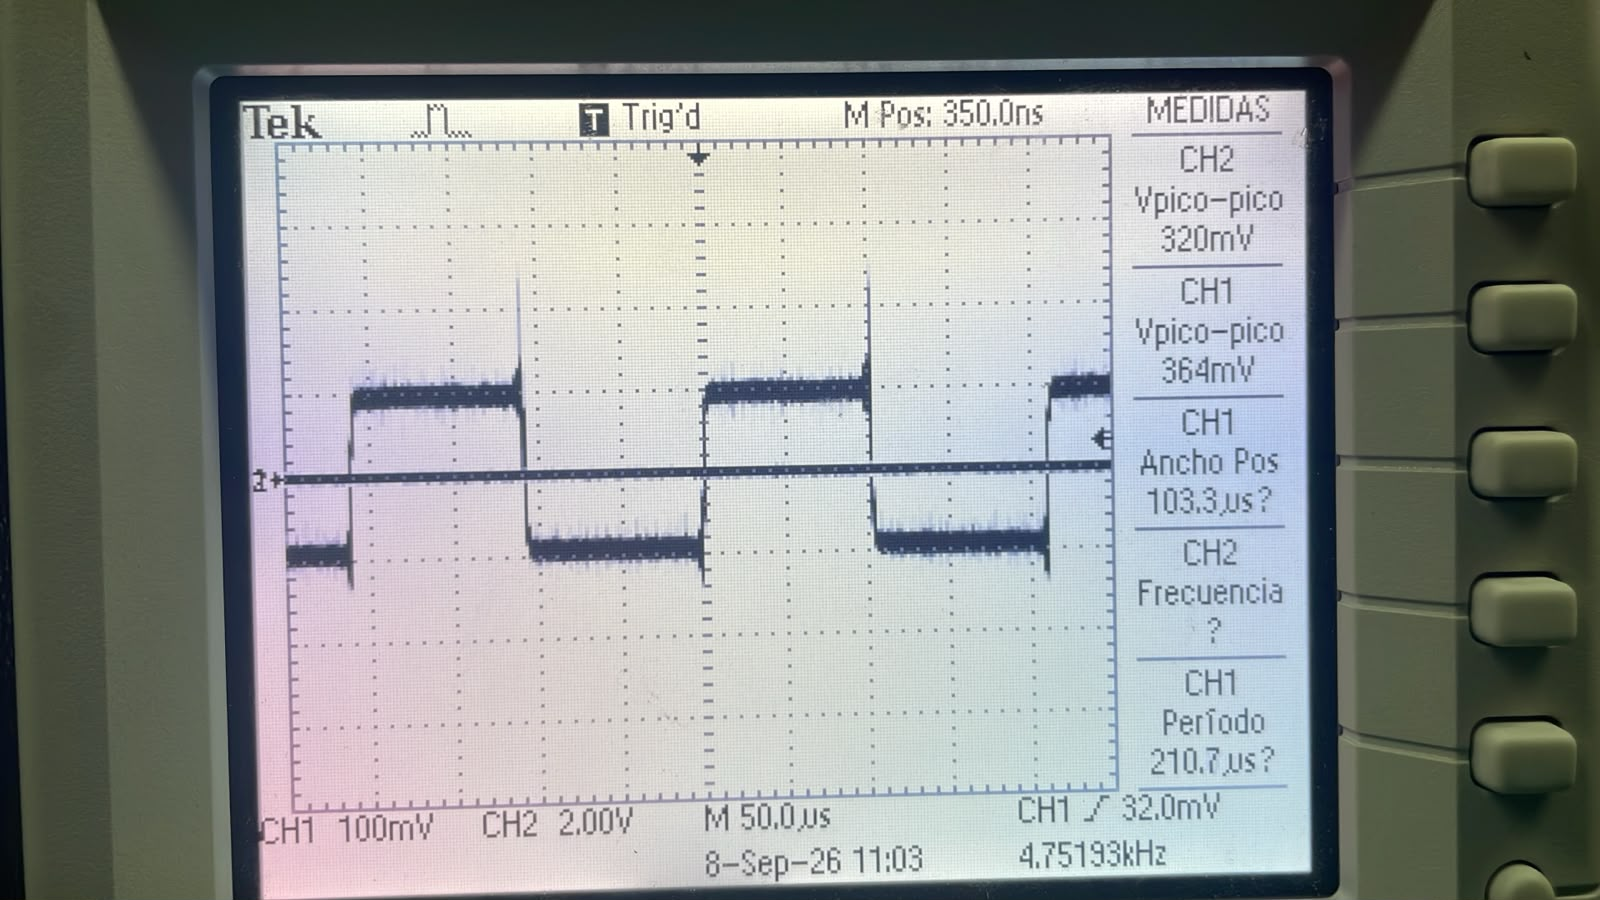
\includegraphics[width=\textwidth]{umbral.png}\\
      \small CH1 (TX): 364 mV$_{pp}$ \quad CH2 (RX): sin señal
    \end{column}
  \end{columns}
\end{frame}

% =====================================================
\section[Conclusiones]{Conclusiones}
\begin{frame}{Conclusiones}
  \begin{itemize}
    \item La \textbf{fibra óptica} entrega mucha más potencia al receptor que el espacio libre, gracias a la reflexión total interna.
    \item El infrarrojo se comporta como la luz visible: puede reflejarse y redirigirse con un espejo.
    \item En modo digital, el receptor funciona como un \textbf{comparador}: regenera la señal si supera el umbral.
    \item Al aumentar la atenuación, la señal puede quedar por debajo del umbral y se pierde la comunicación: el \textbf{balance de potencia} entre emisión, atenuación y sensibilidad es fundamental.
    \item El sistema tiene un \textbf{ancho de banda limitado}: acoplamiento en alterna en baja frecuencia y capacitancias en alta frecuencia.
  \end{itemize}
\end{frame}

\begin{frame}
  \centering
  \Large ¡Gracias!
\end{frame}

\end{document}
